\documentclass[12pt,a4paper]{article}
\usepackage[margin=1in]{geometry}
\usepackage[utf8]{inputenc}
\usepackage{graphicx}
\usepackage{caption}
\usepackage[none]{hyphenat}
\usepackage{hyperref}
\usepackage[nameinlink]{cleveref}

\setlength{\fboxrule}{2pt}

\begin{document}
	\begin{titlepage}
		
		\begin{center}
			
\includegraphics[width=0.5\textwidth]{QUT.jpg}\\
			[0.03\textheight]  
			\Large\textbf{Bachelor of IT (Computer Science)}\\
			\Large\textbf{Assignment 2 - Creative Coding Project}\\
			\large\textbf{DXB211 - Creative Coding}\\
			[0.02\textheight]
			\large\textsl{Dane Madsen}\\
			\large\textsl{n10983864@qut.edu.au}
		\end{center}
		
	\end{titlepage}
	\tableofcontents
	\newpage

	\section{Introduction}
		In WWII Germany, Enigma was an instrumental tool in the German war effort. 
		Enigma was a machine used to encrypt and decrypt intelligence communications 
		between German forces. The sketch created for this assignment aims to simulate 
		the Enigma machines encryption and decryption process.\\
		\\
		To run this sketch you will need to run \texttt{python -m http.server} in the 
		\texttt{src} folder of the project. Then navigate to \texttt{localhost:8000} 
		in your web browser and open the \texttt{entry.html} file.\\
		\\
		To use the sketch, set the three rotors to the desired positions, then simply 
		type and plain text will be displayed next to the \texttt{Input} heading along 
		with the encrypted / decrypted text next to the \texttt{Encoded / Decoded} 
		heading.\\

		\begin{center}
			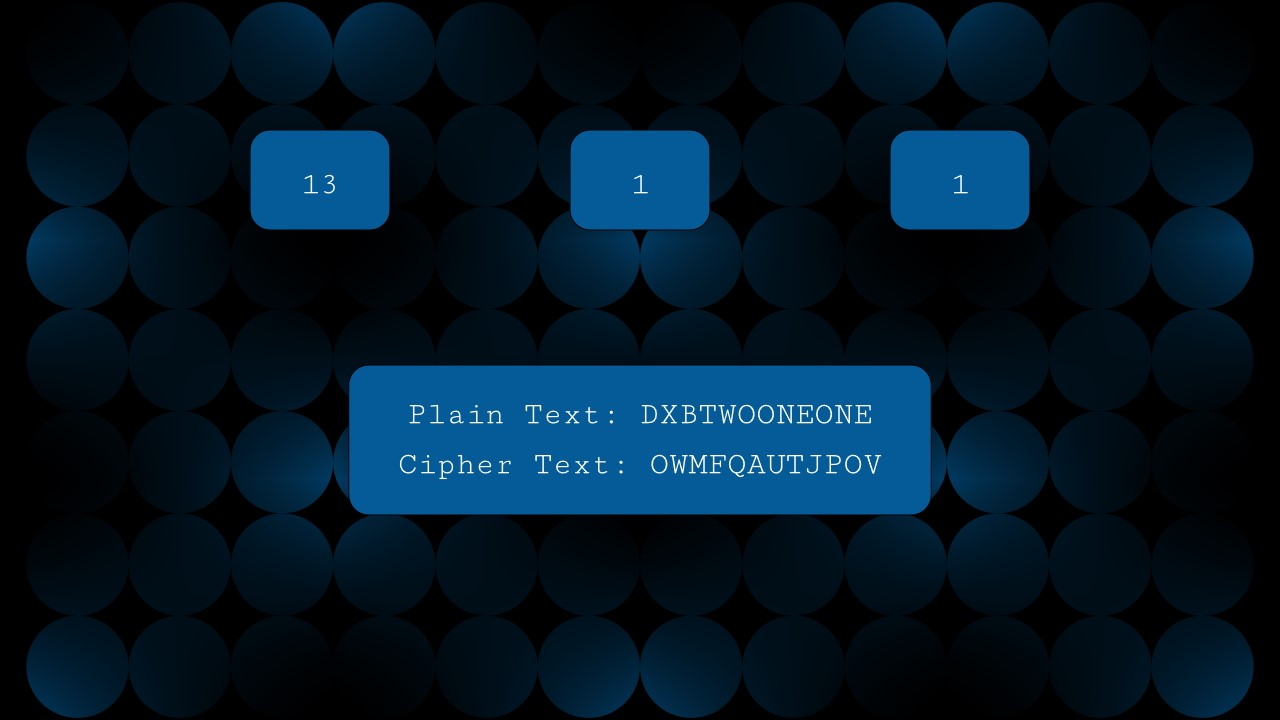
\includegraphics[width=0.8\textwidth]{figures/figure1.jpg}\\
			\vspace{0.5cm}
			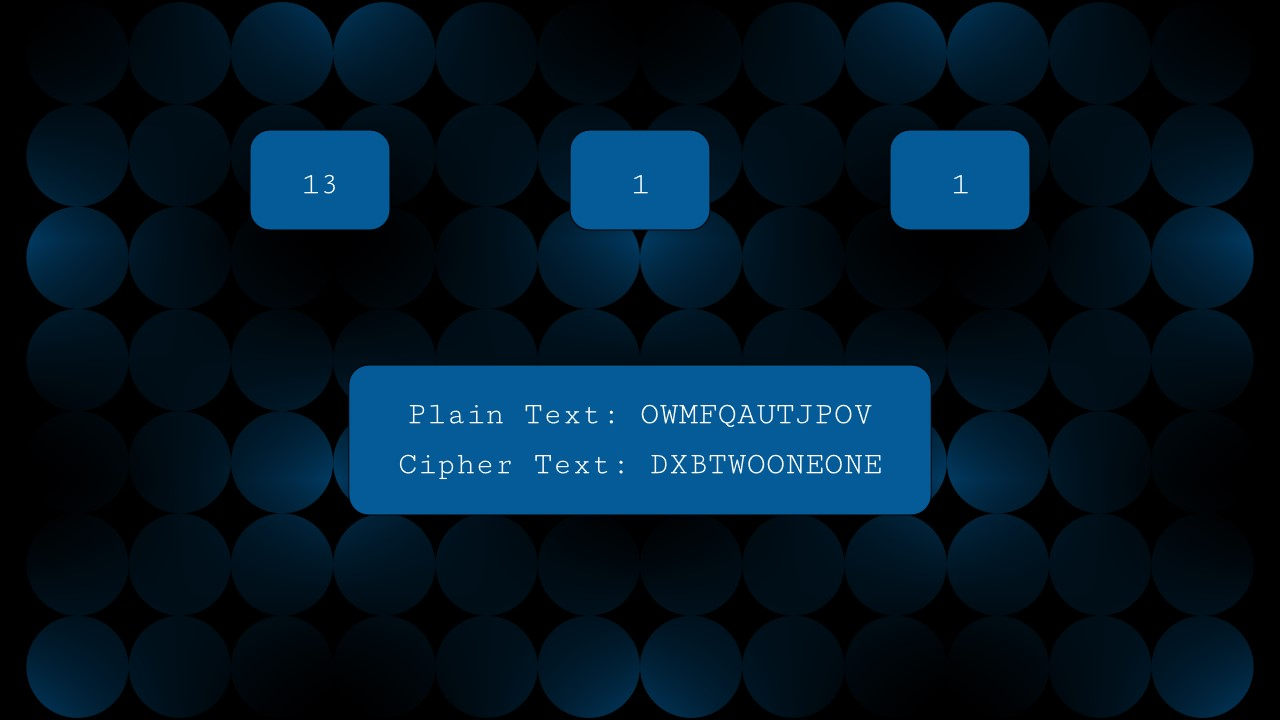
\includegraphics[width=0.8\textwidth]{figures/figure2.jpg}\\
		\end{center}
	
	\newpage

	\section{Design and Aesthetic}
		The sketch has been designed to roughly resemble the style of the 
		\href{https://www.asd.gov.au/}{Australian Signals Directorate (ASD)} website. 
		The ASD is the intelligence agency of Australia responsible for conducting 
		signals intelligence on behalf of the Australian Government. As such, 
		cryptography is highly relivant to the ASD's work.\\

		\begin{center}
			\fbox{
\includegraphics[width=0.8\textwidth]{figures/figure3.jpg}}\\
		\end{center}

\end{document}